\chapter{Integration}
\section{The basic idea}
If we have a distance-time graph, the gradient of the graph gives us the velocity at that point. In the previous chapter, we learnt how to
find the gradient at a point on a curve.

If we have a velocity-time graph, the area under the curve gives us the distance travelled. In this chapter, we will learn how to find this.

The method of finding the area under a curve is called \textbf{integration}.
We will write the area under a curve $y=f(x)$ between $x=a$ and $x=b$ as \[\int_a^b f(x) \dx.\]

\begin{figure}[H]
    \includegraphics[scale=0.75]{img/integration-shaded-graph}
    \centering
  \caption{$\int_a^b f(x) \dx.$}
\end{figure}

\subsection{Finding the area under a curve}
To find the area under a curve, we begin in a similar way to how we began differentiation:

\begin{itemize}
\item[1.] We divide the interval $a\le x\le b$ into small pieces, each of length $h$. 
\item[2.] We build a rectangle on each piece, where the top touches the curve.
\item[3.] We calculate the total area of the rectangles.
\end{itemize}

As we make $h$ get smaller and smaller, the area of the rectangles gets closer and closer to the area under the curve.

\begin{example}
Consider the function $f(x)=x$ on the interval $0\le x\le 1$.

We divide $[0,1]$ into $n$ equal pieces, each of width $h=\frac{1}{n}$. The divisions occur at 
\[0,\frac{1}{n},\frac{2}{n},\dots,\frac{k-1}{n},\frac{k}{n},\dots,\frac{n-1}{n},1\]
or
\[0,h,2h,\dots,n-1)h,1\]

\begin{figure}[H]
\centering
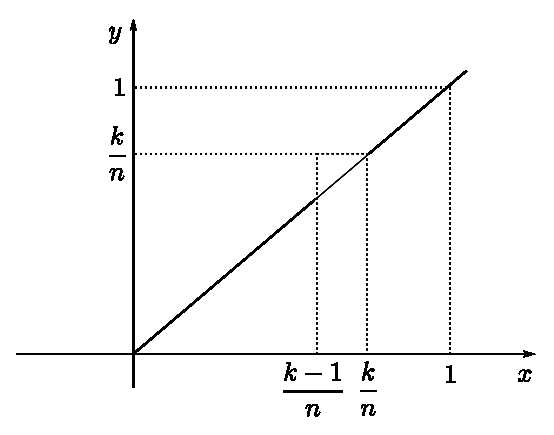
\includegraphics[scale=0.8]{img/graph-x-integration}
\captionstyle{\centering\it}
\caption{The rectangle between $(k-1)h$ and $kh$.}
\end{figure}


The rectangle between $(k-1)h$ and $kh$ will have height $f(kh)=kh$, and the area of this rectangle is
\[\underbrace{kh}_{\text{height}}\cdot\underbrace{h}_{\text{width}}=kh^2.\]

The sum of the area of all rectangles on the interval is
\begin{eqnarray*}
h^2+2h^2+\dots+nh^2 &=& h^2(1+2+\dots+n) \\
&=& h^2\frac{n(n+1)}{2} \\
&=& h^2\frac{\frac{1}{h}(\frac{1}{h}+1)}{2} \\
&=& \frac{1+h}{2}.
\end{eqnarray*}
As $h\to0$, $\frac{1+h}{2}\to \frac{1}{2}$. Therefore, \[\int_0^1 x\dx = \frac{1}{2}.\]
\end{example}

As we did with differentiation, we would like to find faster methods of finding the area under a curve. To do this, we relate integration and differentiation.

\subsection{The fundamental theorem of calculus}
It is often treated as obvious that integration and differentiation are opposites. However, it is un-obvious enough that mathematicians have a big
theorem about it:
\begin{theorem}[Fundamental Theorem of Calculus]
\[\int_a^b g'(x) \dx = g(a)-g(b)\]
\end{theorem}

In other words, if we are trying to find
\[\int_a^b f(x)\dx\]
then if we can find a function $F(x)$ so that $F'(x)=f(x)$,
\[\int_a^b f(x)\dx=F(b)-F(a).\]

\begin{definition}
We call $F(x)$ the \textbf{antiderivative} of $f(x)$.
\end{definition}

The aim of this chapter is to learn methods for finding the antiderivative.

\subsection{Indefinite and definite integrals}

Let $f(x)$ be a function. If $F(x)$ is the antiderivative of $f(x)$, then $F(x)+4$ is also the antiderivative of $f(x)$.
\begin{proof}
\begin{align*}
\frac{d}{dx}\left(F(x)+4\right)&=\frac{d}{dx}\left(F(x)\right)+\frac{d}{dx}\left(4\right)\\&=f(x)+0
\end{align*}
\end{proof}

Similarly, $F(x)+c$ will be the antiderivative of $f(x)$ for any $c\in\mathbb{R}$. When finding an integral without limits, we must include this
constant term.

\begin{definition}
The \textbf{indefinite integral} of a function $f(x)$ is \[\int f(x)\dx = F(x) + c\]
where $F(x)$ is any derivative of $f(x)$. Ususally, we pick $F(x)$ as the antiderivative without a constant term.
\end{definition}
\begin{definition}
\[\int_a^b f(x)\dx = F(x)\] is called the \textbf{definite integral}.
\end{definition}

\section{Finding integrals}

\subsection{Polymonials and other powers}
To find indefinite integrals, we are going to look for functions which will have the correct derivative.

\begin{in_a_box}
\[\int ax^b\dx=\frac{ax^{b+1}}{b+1}+c\]
\begin{proof}
\[\frac{d}{dx}\left(ax^B\right) = aBx^{B-1}\]
so
\[\frac{d}{dx}\left(\frac{ax^B}{B}\right) = ax^{B-1}.\]
Replacing $B$ with $b+1$ gives the correct result.
\end{proof}
\end{in_a_box}

\begin{example}
$$\int x^2\dx = \frac{x^3}{3}+c$$
\end{example}
\begin{example}
$$\int x^2+x^3\dx = \frac{x^3}{3}+\frac{x^4}{4}+c$$
\end{example}
\begin{example}
To find
$$\int_0^x t^2\dx[t],$$
or the area under $y=t^2$ between $t=0$ and $t=x$:
\begin{figure}[H]
\centering
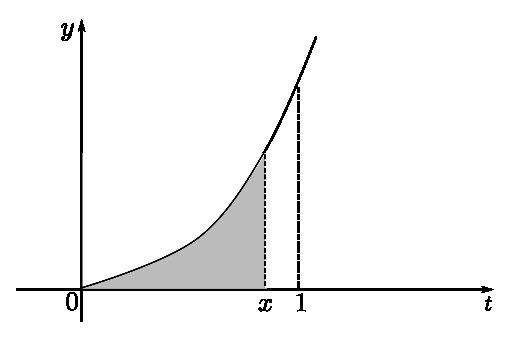
\includegraphics[scale=0.8]{img/integration-graph-t-squared}
\end{figure}

We first find
$$\int t^2\dx[t] = \frac{t^3}{3}+c.$$
Then
\begin{align*}\int_0^x t^2\dx[t] &= \frac{x^3}{3}+c-\frac{0^3}{3}-c\\&=\frac{x^3}{3}.\end{align*}

For $x=1$, the area under $y=t^2$ between $t=0$ and $t=1$ is
\begin{align*}\int_0^1 t^2\dx[t] &=\frac{1^3}{3}\\&=\frac{1}{3}.\end{align*}

\end{example}

When finding definite integrals, the constants will always cancel, so can be ignored. We often write the working like this, with the indefinite integral in brackets:

\begin{example}
\begin{align*}
\int_1^3 3x^2\dx&=\left[x^3\right]_1^3\\
&=3^3-1^3\\
&=26
\end{align*}
\end{example}

This also works with negative and fractional powers.

\begin{example}
Suppose we want to integrate the function $1/x^2$ over the interval $[1,2]$. That is, we want to calculate
\[\int_1^2 \frac{1}{x^2}\dx.\]
If we put $F(x)=-1/x$, then 
\[F'(x)=\frac{d}{dx}\left(-\frac{1}{x}\right)=\frac{1}{x^2}.\]
So we can write
\[\int_1^2\frac{1}{x^2}\dx=\left[-\frac{1}{x}\right]_1^2=\left(-\frac{1}{2}\right)-\left(-\frac{1}{1}\right)=\frac{1}{2}.\]
The integral $\int_1^2\frac{1}{x^2}\dx$ represents the area under the curve $y=\frac{1}{x^2}$ between 1 and 2, therefore we understand that this integral makes some geometrical sense.

\begin{figure}[H]
\centering
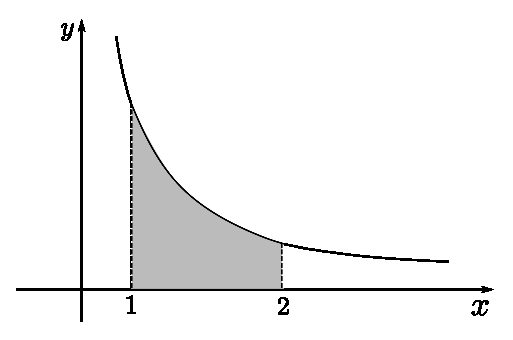
\includegraphics[scale=0.8]{img/integration-graph-over-x-squared}
\caption{Integrating to find the shaded area under the curve $y=\frac{1}{x^2}$ on the interval $[1,2]$.}
\end{figure}
\end{example}

\begin{example}
\begin{align*}
\int \sqrt{x}\dx&=\int x^\frac{1}{2}\dx\\
&=2x^\frac{3}{2}+c
\end{align*}
\end{example}

$x^{-1}$ is a special case, as using the same rule would require division by 0:

\begin{in_a_box}
\[\int \frac{1}{x}\dx = \ln |x|+c\]
\begin{proof}
This is true because for $x>0$
\[\frac{d}{dx}(\ln x)=\frac{1}{x},\]
and for $x<0$,
\[\frac{d}{dx}(\ln |x|)=\frac{d}{dx}(\ln (-x))=\frac{-1}{-x}=\frac{1}{x}.\]
\[\frac{d}{dx}\ln x=\frac{1}{x}.\]
\end{proof}
\end{in_a_box}



\subsection{Exponential functions}

\begin{in_a_box}
\[\int e^x\dx = e^x+c\]
\begin{proof}
This is true because \[\frac{d}{dx}e^x=e^x.\]
\end{proof}
\end{in_a_box}

\begin{in_a_box}
\[\int a^x\dx = \frac{a^x}{\ln a}+c\]
\begin{proof}
This is true because 
\begin{align*}
\frac{d}{dx}\left(\frac{a^x}{\ln a}\right)&=\frac{1}{\ln a}\frac{d}{dx}\left(e^{x\ln a}\right)\\
&=\frac{1}{\ln a}e^{x\ln a}\ln a\\
&=e^{x\ln a}.
\end{align*}
\end{proof}
\end{in_a_box}


\subsection{Trigonometric functions}
\begin{in_a_box}
\[\int \cos x\dx=\sin x + c,\quad\quad \text{since }\frac{d}{dx}(\sin x)=\cos x,\]
\end{in_a_box}
\begin{in_a_box}
\[\int \sin x\dx=-\cos x + c,\quad\quad \text{since }\frac{d}{dx}(-\cos x)=\sin x.\]
\end{in_a_box}


\section{Rules for integration}
Instead of making a longer and longer list of functions and their antiderivatives, we are going to learn some rules for integration and use these
to work out harder integrals

\subsection{Sum rule and constants}
\begin{thing}{Sum Rule}
\begin{equation}
\int \left( f(x)+g(x) \right)\dx=\int f(x)\dx+ \int g(x)\dx
\end{equation}
\end{thing}
\begin{thing}{Multiplication by a constant}
\begin{equation}
\int K f(x)\dx=K\int f(x)\dx
\end{equation}
\end{thing}
Both these rules follow from the equivalent rules differentiation.

